\subsection{Overview}
\label{sec:frontend_overview}

The Gateway Dashboard is a modern web application built with Vue.js 3, providing an intuitive management interface for the Speech Gateway API. The application supports user authentication, subscription management, and administrative controls through a responsive single page application architecture.

\subsubsection{Frontend Architecture}

Figure~\ref{fig:frontend_architecture_simple} illustrates the layered architecture of the frontend application, showing the four main layers and how data flows between them.

\begin{figure}[H]
\centering
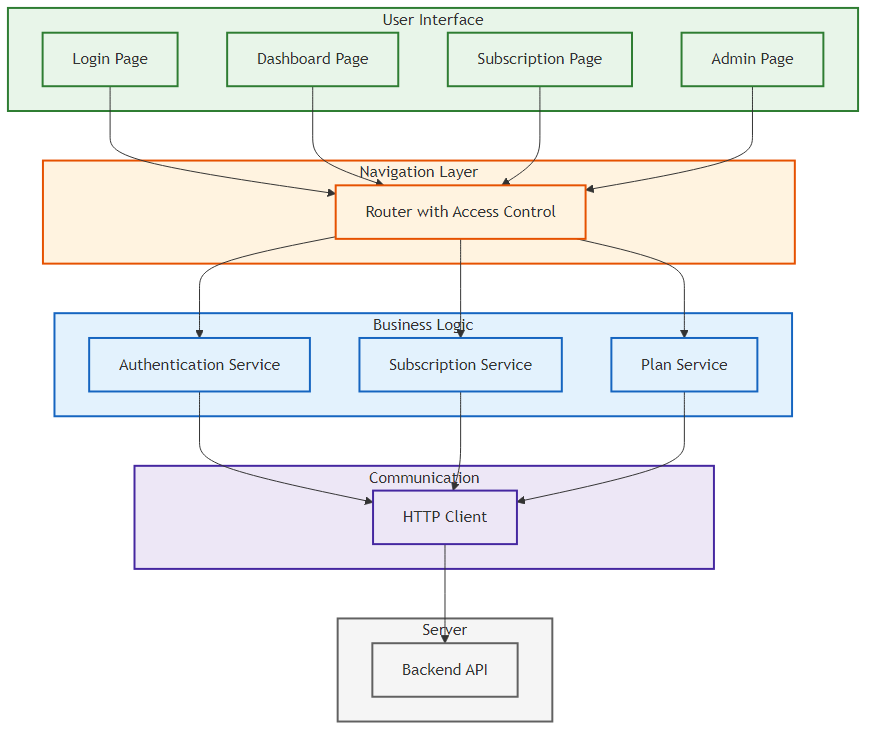
\includegraphics[width=0.8\textwidth]{images/frontend_architecture_simple.png}
\caption{Frontend Application Architecture}
\label{fig:frontend_architecture_simple}
\end{figure}

The frontend follows a clean layered architecture with clear separation of concerns. At the top, the \textbf{User Interface} layer contains the pages that users interact with (Login, Dashboard, Subscription, and Admin). The \textbf{Navigation} layer manages which pages users can access based on their authentication status and role. The \textbf{Business Logic} layer handles authentication state, subscription data, and plan information. At the bottom, the \textbf{Communication} layer sends and receives data from the backend API, automatically attaching authentication credentials to every request.

This layered approach ensures that changes in one layer (for example, updating the UI design) do not affect the underlying business logic or communication mechanisms.

\subsubsection{Technology Stack}

\begin{table}[H]
\centering
\begin{tabular}{|l|l|}
\hline
\textbf{Layer} & \textbf{Technology} \\
\hline
Frontend Framework & Vue.js 3 \\
\hline
UI Component Library & Vuetify (Material Design 3) \\
\hline
Build Tool & Vite \\
\hline
Routing & Vue Router 4 \\
\hline
\end{tabular}
\caption{Frontend Technology Stack}
\label{tab:frontend_tech_stack}
\end{table}

The application uses Vue.js 3 as the core framework for building reactive user interfaces. Vuetify provides a comprehensive set of Material Design components, ensuring a professional and consistent user experience. Vite serves as the build tool, enabling fast development and optimised production builds. Vue Router 4 manages navigation and enforces authentication constraints through navigation guards.
